\documentclass[12pt]{article}

\usepackage[utf8]{inputenc}
\usepackage[margin=1in]{geometry}
\usepackage[titletoc,title]{appendix}
\usepackage[section]{placeins}  % allows us to stop floaters
\usepackage{longtable}  % for bringing in our data tables to the appendix
\usepackage{amsmath,amsfonts,amssymb,mathtools}
\usepackage{graphicx,float}
\usepackage{makecell}
\usepackage{caption}
\usepackage{csvsimple,booktabs} % load csv data into table
\usepackage{filecontents} % read csv data contents
\usepackage{indentfirst} % set first paragraph of each section to be indented
\usepackage[backend=biber,style=authoryear]{biblatex} % style our references

\addbibresource{references.bib} % load resources from bib file
\setlength{\parindent}{1.5em} % set indent length for each paragraph
\graphicspath{ {../figures/} }

\newcommand*\mean[1]{\overline{#1}}

\title{Fire and Ice\\
\large Volcanism and the Ice-Albedo Feedback}
\author{
    E. Giroud-Proeschel - 52917770 \\
    P. Matlashewski - 45701109\\
    M. Ormerod - 16265167
}

\begin{document}

\maketitle
\centerline{Word Count: 2456}
\newpage
\tableofcontents
\newpage

% Introduction and Overview
\section{Introduction}
Earth's past is marked by extreme climate variations, with evidence of
reversals between hothouse and coldhouse regimes. A possible driving force behind
these reversals is volcanism. In this study, we focus on
how large volcanic out-gassing of volatiles such as sulfur dioxide,
affect the Earth's climate. Here we chose to investigate
the impact of volcanic perturbations on a simple radiative
energy balance model. Throughout this paper we will only consider the effect of aerosols,
and more specifically, SO2. This model is inspired by the
work of Russian climatologist Mikhail I. Budyko, who discovered the ice-albedo
feedback mechanism through his pioneering of studies
on global climate using physical models of temperature equilibrium \parencite{budyko_albedo}.
We proceed as follows:

\begin{enumerate}
    \item Build a graphical algorithm solving the radiative energy balance equations
    in a zonally-averaged Earth model (section \ref{sec:algorithm}).
    \item Compute a steady-state energy balance of the Earth to investigate
    the effects of inter-zonal transfer by:
    \begin{enumerate}
        \item setting all transfer coefficients $k_{ij}$ to zero and finding the
        equilibrium temperature distribution.
        \item using the provided values of $k_{ij}$ and comparing heat transfer
        magnitudes and rates from our previous step.
    \end{enumerate}
    \item To investigate the cooling effects of volcanism, we use data from
    the 1982 El Chichón and Pinatubo eruptions \parencite{robock}
    to characterize the spatially and temporally reducing effects of stratospheric aerosols
    on incoming solar radiation.
    \item To parameterize the intensity volcanic cooling, we model the frequency
    of volcanic eruptions as a Poisson process.
    \item To consider the possibility of a coldhouse regime (or snowball Earth),
    we introduce an ice-albedo feedback using temperature-dependent zonal albedos.
    \item Finally, we combine the cooling effects of volcanism combined with the
    ice-albedo feedback model to investigate if volcanic activity
    can give rise to a snowball Earth scenario.


\end{enumerate}

\subsection{Budyko Climate Model}
The evolution of Earth's temperature will be investigated using a Budyko
climate model \parencite{budyko_albedo}. The earth is divided into 6 latitudinal
zones, defined in table \ref{tab:latitudes} and figure \ref{fig:zones}
\parencite{jellinek_ps}.

\begin{table}
    \centering
    \begin{tabular}{ c | c | c }
        \hline
        \thead{Zone} & 
        \thead{Lower Latitude} &
        \thead{Upper Latitude} \\
        \hline
        1 & $90^\circ S$ & $60^\circ S$ \\
        2 & $60^\circ S$ & $30^\circ S$ \\
        3 & $30^\circ S$ & $0^\circ$ \\
        4 & $0^\circ$ & $30^\circ N$ \\
        5 & $30^\circ S$ & $60^\circ N$ \\
        6 & $60^\circ S$ & $90^\circ N$ \\
        \hline
    \end{tabular}
    \caption{Zone latitudes.}
    \label{tab:latitudes}
\end{table}

\begin{figure}[H]
    \centering
    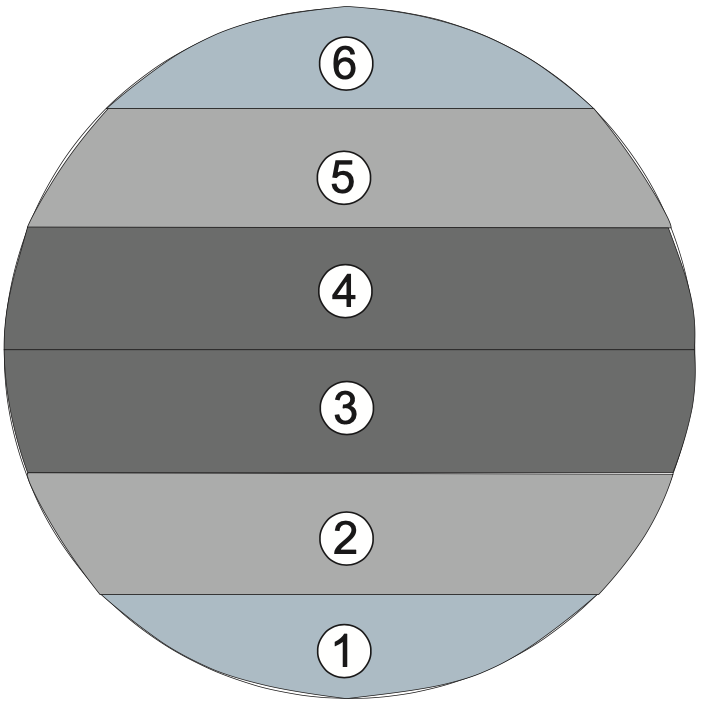
\includegraphics[scale=0.3]{zones.png}
    \caption{Latitude zone intervals.}
    \label{fig:zones}
\end{figure}
\FloatBarrier

Within each zone, temperature evolves through a balance of incoming solar radiation,
outgoing long-wave radiation and the exchange of heat between zones.
These effects are quantified through
\begin{equation} \label{eqn:budyko}
    \frac{dT_k}{dt} = \frac{1}{\mean{\rho_kc_k[Z_k]}}
    \{
      \gamma_k(1-\alpha_k^{sky})(1-\Bar{\alpha}_k)S_0-\tau\sigma_BT_k^{4}
    \} +
    \frac{L_{ki}k_{ki}}{{A_k}\mean{\rho_kc_k[Z_k]}}(T_{k}-T_{i})
\end{equation}
where $k = 1,\dots,6$ represents each latitudinal zone and $T_k$ is the zonal
temperature. The remaining constants are defined in tables \ref{tab:zoneparams}
and \ref{tab:globalparams} of section \ref{sec:Parameters}.

\subsection{Volcanic Eruptions} \label{sec:Volcanos}
Volcanism is an important natural cause of climate change on both short and long-term
timescales \parencite{robock}. For our investigation, we consider the
short-term cooling effects of volcanism that occur on a $10-100$ year time frame.
A zonal occlusion factor, $\phi_k(t)$, introduces this cooling effect to our model
(equation \ref{eqn:occlusion}). The occlusion factor represents volcanic aerosols
suspended in the atmosphere that block direct shortwave solar radiation.
\begin{equation} \label{eqn:occlusion}
\frac{dT_k}{dt} = \frac{1}{\mean{\rho_kc_k[Z_k]}}
\{
    \phi_k(t)\gamma_k(1-\alpha_k^{sky})(1-\Bar{\alpha}_k)S_0-\tau\sigma_BT_k^{4}
\} +
\frac{L_{ki}k_{ki}}{{A_k}\mean{\rho_kc_k[Z_k]}}(T_{k}-T_{i})
\end{equation}
A value of $\phi(t) = 1$ represents no volcanic aerosol occlusion. A value
of $\phi(t) = 0.7$, for example, represents a $30\%$ reduction in total
incoming solar radiation.

\subsubsection{Direct Radiation Occlusion} \label{sec:Occlusion}
The function $\phi(t)$ was fit to observations of reduced solar radiation following the
1982 El Chichón eruption and the 1991 Pinatubo eruption \parencite{robock} (figure
\ref{fig:occlusion}). We found that a function with the form
$\phi(t) = 1 - ct^{-2}$, where $c=5.36$ yr$^2$ is an empirical constant found through
nonlinear regression, gave a reasonable representation of the data.
This function has the property that $\phi(t) \to 1$ as $t \to \infty$,
which models the decaying effects of aerosol occlusion over time.

\begin{figure}[H]
    \centering
    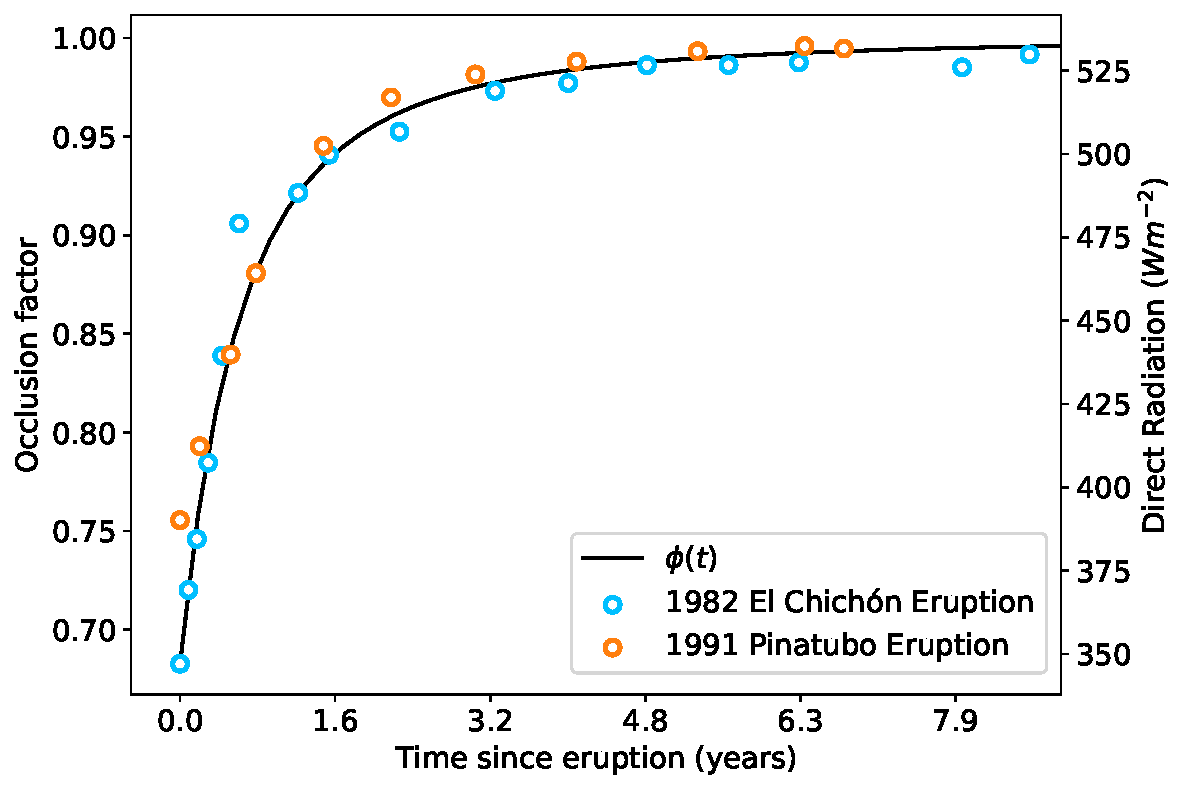
\includegraphics[scale=0.6]{occlusion.pdf}
    \caption{
        A plot of the empirically fit occlusion function.
    }
    \label{fig:occlusion}
\end{figure}
\FloatBarrier

\subsubsection{Spatial Distribution of Aerosols} \label{sec:Spatial_Occlusion}
The effects of a volcanic eruption are not restricted to a single zone. Suspended
aerosols are dispersed throughout the atmosphere and can travel large distances
across the Earth. To model the spatial effects of aerosol dispersion following
an eruption, a time lag is introduced to the zonal occlusion functions,
$\phi_k(t)$, that varies based on the distance zone $k$ is from the eruption
zone. An example is shown in figure \ref{fig:occlusion_space}, where an eruption
occurs at $t=0$ in zone $1$. For the first $3$ months following the eruption,
only zone 1 has the occluding effects of volcanic aerosols. After $3$ months,
the aerosols have traveled to the adjacent zone 2, where $\phi_2(t)$ begins
to follow the decaying occlusion function defined in section \ref{sec:Occlusion}.
Global coverage occurs after approximately 9 months. The specific lag times considered
were estimated from the data presented in \cite{robock}.

\begin{figure}[H]
    \centering
    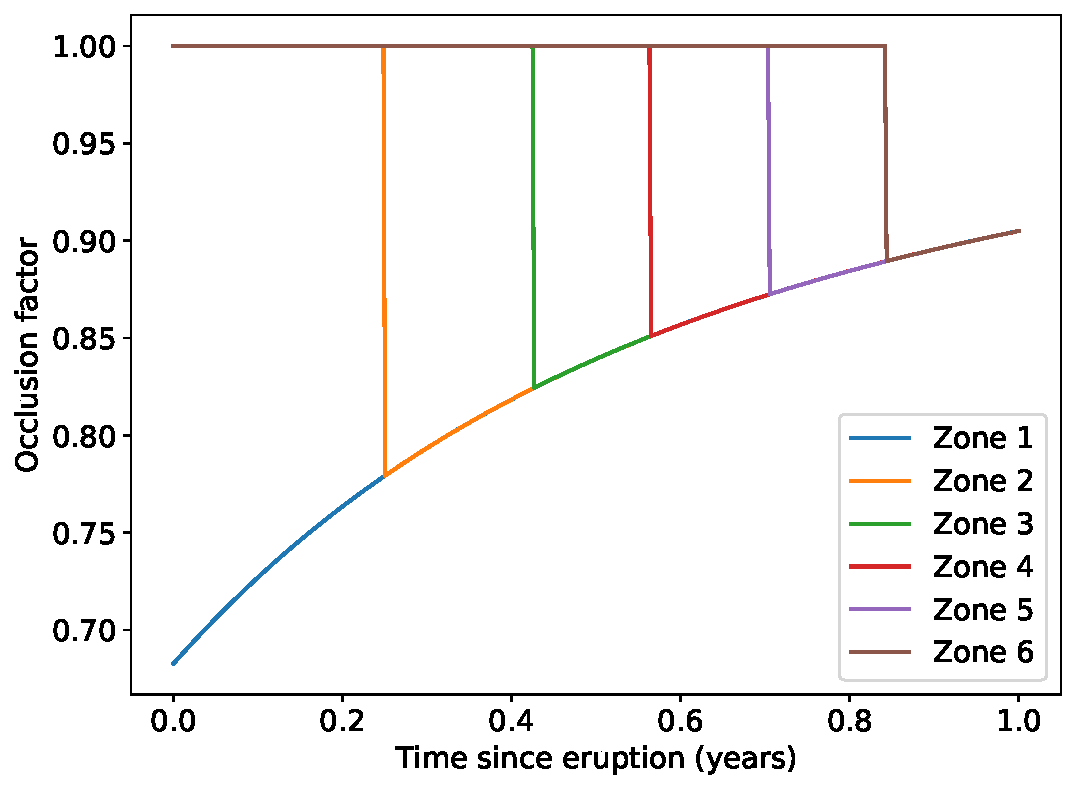
\includegraphics[scale=0.6]{occlusion_space.pdf}
    \caption{
        The spatial effect of eruptions. A distance-dependent time lag is
        present for zones adjacent to the eruption.
    }
    \label{fig:occlusion_space}
\end{figure}
\FloatBarrier

\subsubsection{Stochastic Eruption Frequency} \label{sec:Stochastic}
Sections \ref{sec:Occlusion} and \ref{sec:Spatial_Occlusion} define our model's
response to a single eruption. To investigate the intensity of
volcanism on the Earth's climate, we allow for a series of eruptions to occur
over time. Volcanic eruptions in each zone are modeled as a Poisson
process, where each zone is prescribed an eruption frequency parameter,
$\lambda_k$, reflecting the average repose time between eruptions in the zone.
For an eruption frequency $\lambda_k$, the probability of a repose time, $t_{R}$,
between eruptions follows an exponential distribution
\begin{equation} \label{eq:exponential}
P(t_{R}) = \lambda_k e^{-\lambda_k t_{R}}
\end{equation}
For this investigation, we assume eruptions occur independently between zones. \\

The intensity of volcanic activity on Earth can be adjusted through
$\lambda_k$. A smaller $\lambda_k$ represents shorter repose
times and higher volcanic activity. Combining equation \ref{eq:exponential} with
the occlusion function defined in sections \ref{sec:Occlusion} and
\ref{sec:Spatial_Occlusion} gives a simple stochastic model for volcanism on
Earth that includes the time-decaying effects of aerosol occlusion, the spatial
dispersion of aerosols and eruption frequency.

\subsection{Ice-Albedo Feedback} \label{sec:Ice}
The volcanism defined in section \ref{sec:Volcanos} provides a mechanism to
cool the Earth by occluding direct solar radiation with suspended volcanic
aerosols. One interesting way to study the implications of this cooling is by
considering the ice-albedo feedback \parencite{budyko_albedo}. If the temperature
of the Earth is cold enough, ice will grow and cover a larger proportion of the
Earth's surface. This will result in a higher surface albedo, reflecting more
incoming solar radiation. This further contributes decreasing the temperature of
the Earth, leading to a positive feedback and a potential ``snowball Earth'' scenario.\\

Ice-albedo feedback is modeled by defining a temperature dependent albedo as follows
\begin{equation} \label{eqn:albedoparam}
    \alpha_k(T_k) =
      \begin{cases}
      \alpha_{k0} & T_k \geq T_0 \\
      \alpha_{k0} + (\alpha_i-\alpha_k)\frac{(T_k-T_0)^2}{(T_i-T_0)^2}
      & T_i < T_k < T_0 \\
      \alpha_i & T_k \leq T_i
      \end{cases}
\end{equation}
where $\alpha_k$ is the albedo in zone $k$, $T_k$ is the temperature in
zone $k$, $T_0 = 280$ K is the threshold temperature below which
zonal ice cover will grow to increase the albedo, $T_i = 250$ K is the temperature
where the zone is completely covered in ice, $\alpha_{k0}$ is the baseline
zonal albedo given in table \ref{tab:zoneparams} and $\alpha_i = 0.6$ is the
albedo of ice. Figure \ref{fig:albedotemp} shows the nonlinear albedo function
for each zone.

\begin{figure}[H]
    \centering
    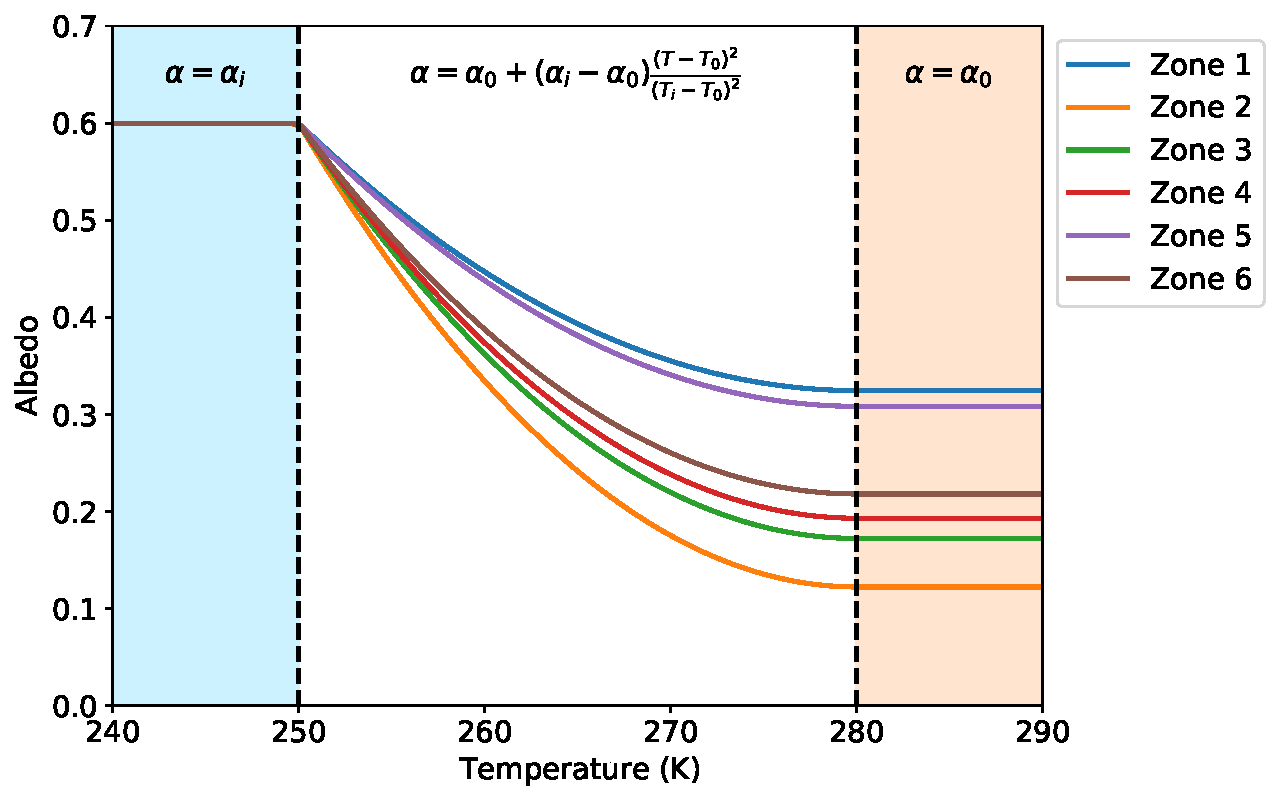
\includegraphics[scale=0.6]{albedo.pdf}
    \caption{
        Albedo parameterization as a function of temperature in each zone.
        The blue shaded region indicates the temperature range where a zone
        is covered with ice. The orange shaded region indicates the temperature
        range where there is no change in ice as temperature varies.
    }
    \label{fig:albedotemp}
\end{figure}
\FloatBarrier

% Figure results
\section{Results}
\label{section:results}

\subsection{Steady-State Climate Model: No Volcanism}
By passing initial condition temperatures calculated through our model with
suppressed inter-zonal transfer (table \ref{tab:teq}) to  our  model  where 
inter-zonal  transfer  is allowed. Figure \ref{fig:steadystate} shows the
equilibrium temperatures for a model where El Niño is neglected (dashed lines)
and where El Niño is considered (solid lines).

\begin{table}[H]
    \centering
    \begin{tabular}{ c | c | c }
        \hline
        \thead{Zone} &
        \thead{Inter-zonal Heat Transfer Suppressed \\ Equilibrium Temperature [K]} &
        \thead{Inter-zonal Heat Transfer Allowed \\ Equilibrium Temperature [K]} \\
        \hline
        1 & 217.23 & 274.12 \\
        2 & 279.74 & 279.34 \\
        3 & 296.45 & 282.26 \\
        4 & 294.56 & 280.88 \\
        5 & 263.56 & 279.71 \\
        6 & 225.33 & 274.93 \\
        \hline
    \end{tabular}
    \caption{
        Equilibrium Temperature distributions for a climate model with no
        volcanism
    }
    \label{tab:teq}
\end{table}

\begin{figure}[H]
    \centering
    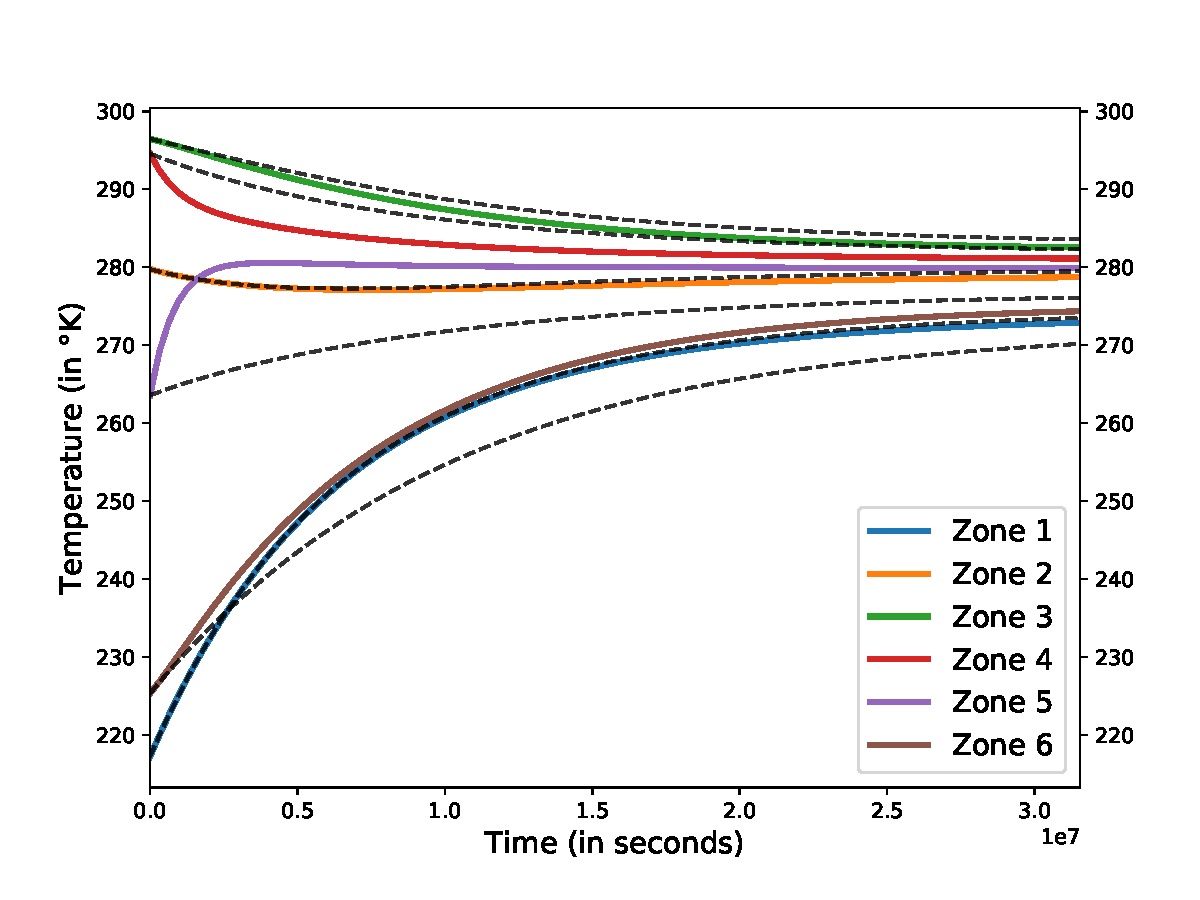
\includegraphics[scale=0.6]{Question2.pdf}
    \caption{
        Equilibrium solution for 6-zoned Earth climate model. Zone 1 marks the
        southernmost band at $60-90^{\circ}$S while zone 6 represents the
        northernmost band at $60-90^{\circ}$N. Zones 2-5 are bands covering
        $30^{\circ}$ intervals between zones 1 and 6
        (See Figure \ref{fig:zones}).
    }
    \label{fig:steadystate}
\end{figure}
\FloatBarrier

\subsection{Climate Model Following Single Volcanic Eruption}
Figure \ref{fig:oneerupt} shows the effect of a single eruption on zonal 
temperatures initially at steady-state. The eruption occurs in zone 4 after
1 year, as indicated by the vertical dashed line.
Zone 4 is immediately affected by the solar occlusion and shows a decrease
in temperature. A time lag between the zonal temperature responses is clearly
visible with zones at a greater distance from zone 4 showing a larger time lag.
The recovery of each zone to its equilibrium temperature occurs over approximately
15 years after the eruption. The equilibrium temperature values are the same
post-eruption as they are pre-eruption.

\begin{figure}[H]
    \centering
    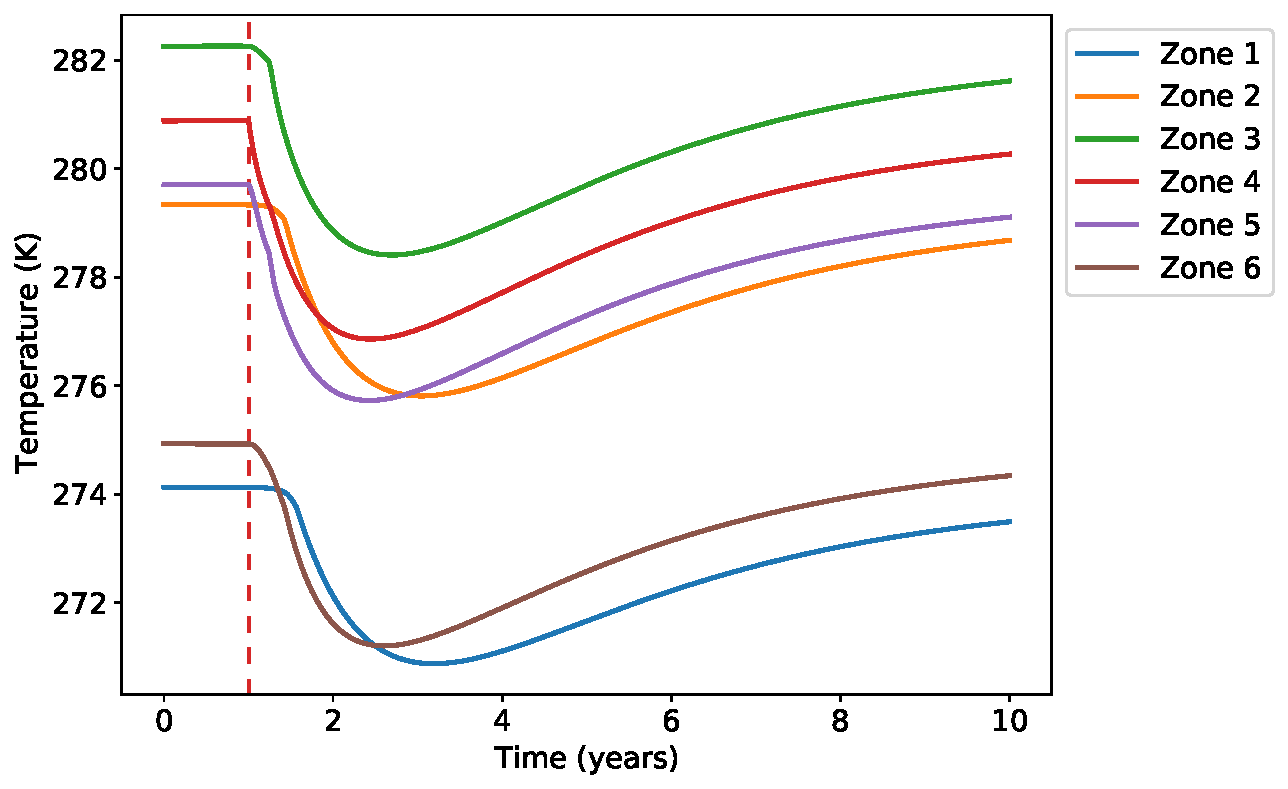
\includegraphics[scale=0.6]{one_eruption.pdf}
    \caption{
        Reduction in solar forcing post eruption results in temperature drop.
    }
    \label{fig:oneerupt}
\end{figure}
\FloatBarrier

\subsection{Stochastic Volcanic Eruptions}
Figure \ref{fig:stocherupt} shows a model result that includes multiple
eruptions following the Poisson process defined in section \ref{sec:Stochastic}.
Vertical dashed lines represent an eruption with a coloured by the zone the eruption
occurred. The eruption intensity parameters used are given in table
\ref{tab:lambda_stochastic}
\begin{table}
    \centering
    \begin{tabular}{ c | c }
      \hline
      \thead{Zone} & 
      \thead{$\lambda_k [\text{yr}^{-1}]$} \\
      \hline
      1 & 100 \\
      2 & 50 \\
      3 & 20 \\
      4 & 20 \\ 
      5 & 50 \\
      6 & 100 \\
    \hline
    \end{tabular}
    \caption{Volcanic intensity rate parameters}
    \label{tab:lambda_stochastic}
\end{table}
\begin{figure}[H]
    \centering
    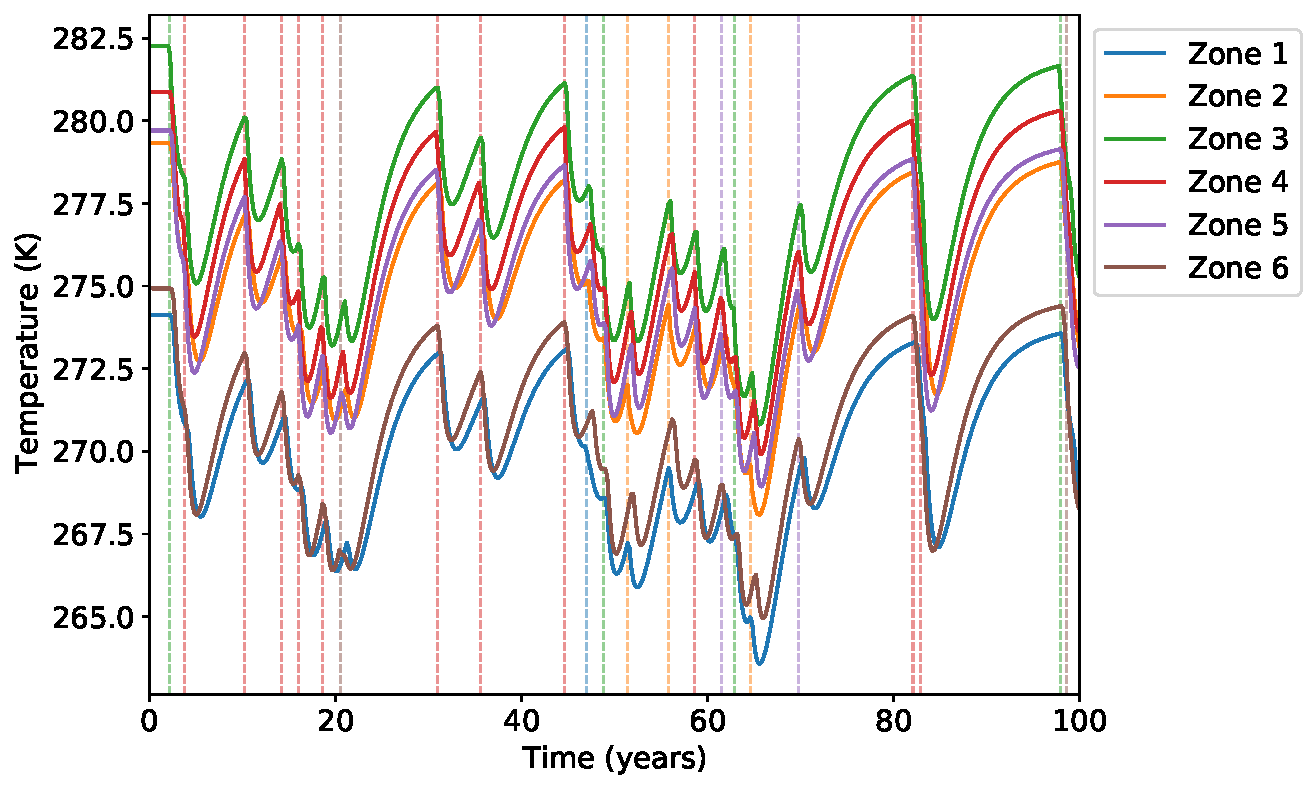
\includegraphics[scale=0.6]{stochastic_eruptions.pdf}
    \caption{
        Stochastic eruption distribution following Poisson distribution.
        Vertical dotted lines are colored based on the zone the eruption
        occurred in, and their placement is the point in time at which the
        eruption is initiated.
    }
    \label{fig:stocherupt}
\end{figure}
\FloatBarrier

The model was run for 100 years to show multiple cycles of temperature
drops and recoveries. From Figure
\ref{fig:stocherupt}, we see that following each eruption is a decline in zonal
temperatures, and sufficiently close eruptions, in time, compound that effect.
The distribution lag associated with aerosol spreading is still represented
numerically, though a lag of a few months is difficult to discern visually on
this extended time scale. 

\subsection{The Ice-Albedo Effect} \label{sec:ice_albedo_results}
Figure \ref{fig:albedo_equil} shows the result of the temperature dependent albedo
from in equation \ref{eqn:albedoparam} coupled with our climate model in
equation \ref{eqn:budyko}. The temperature ranges for the nonlinear albedo model
are coloured similar to figure \ref{fig:albedotemp}. We recognize three temperature equilibria,
two of which are stable and one that is unstable. The equilibrium temperature
distributions are shown in table \ref{tab:eqstates}.

\begin{table}
    \begin{tabular}{ c | c | c | c }
      \hline
      \thead{Zone} & 
      \thead{Warm Earth \\ Equilibrium Temperature [K]} &
      \thead{Unstable \\ Equilibrium Temperature [K]} &
      \thead{Snowball Earth \\ Equilibrium Temperature [K]} \\
      \hline
      1 & 274.02 & 251.08 & 231.91 \\
      2 & 279.27 & 255.03 & 234.30 \\
      3 & 282.21 & 258.31 & 236.23 \\
      4 & 280.83 & 257.78 & 236.13 \\ 
      5 & 279.66 & 256.98 & 235.70 \\
      6 & 274.83 & 253.11 & 233.20 \\
        \hline
    \end{tabular}
    \caption{Ice-albedo effect equilibrium temperature distributions}
    \label{tab:eqstates}
\end{table}

\begin{figure}[H]
    \centering
    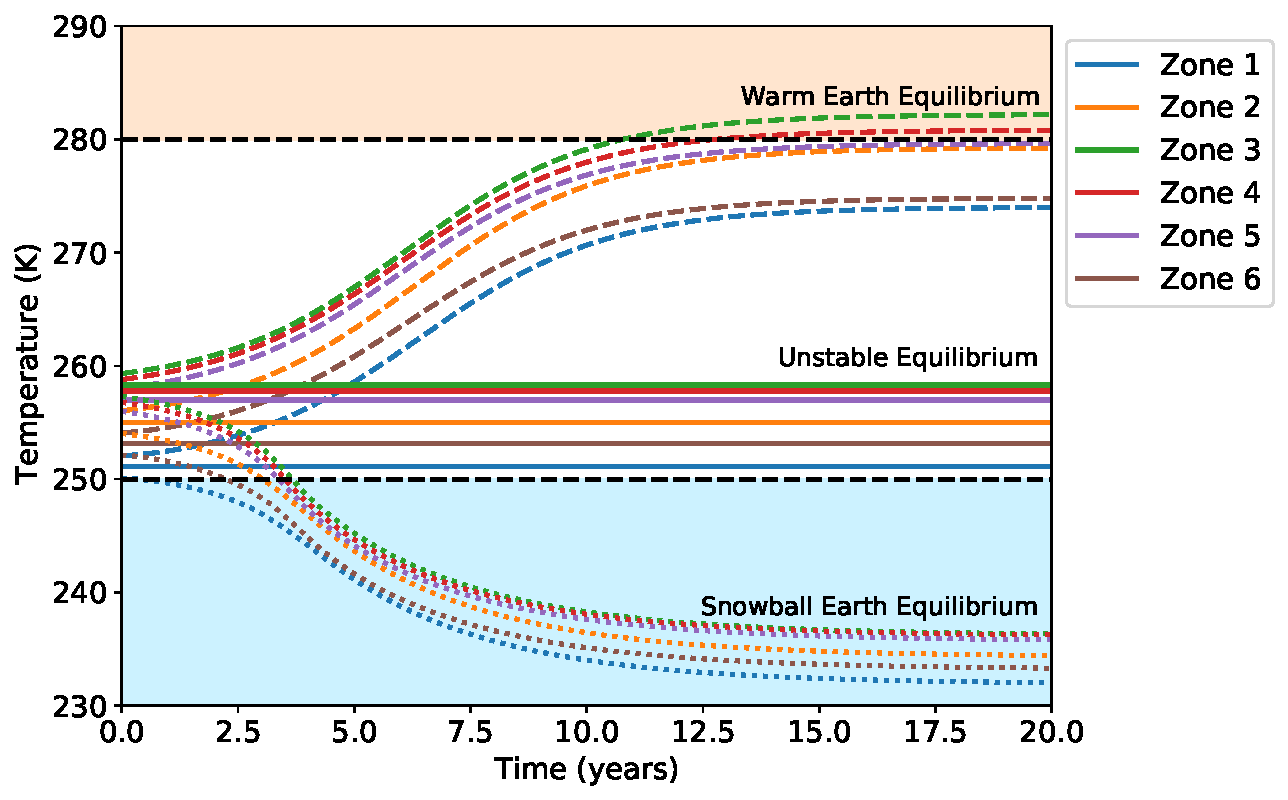
\includegraphics[scale=0.6]{albedo_equilibria_1plot.pdf}
    \caption{
        Integrating through climate model incorporating both stochastic volcanic
        eruptions and ice-albedo feedback parameterization.
    }
    \label{fig:albedo_equil}
\end{figure}
\FloatBarrier

A model started with an initial temperature distribution at the unstable equilibrium
(solid lines in figure \ref{fig:albedo_equil}) remains at the unstable equilibrium. \\

A model started with an initial temperature distribution perturbed slightly above
the unstable equilibrium (dashed lines in figure \ref{fig:albedo_equil}) asymptotically
approaches the ``warm Earth'' equilibrium given in table \ref{tab:eqstates}. \\

A model started with an initial temperature distribution perturbed slightly below
the unstable equilibrium (dotted lines in figure \ref{fig:albedo_equil}) asymptotically
approaches the ``snowball Earth'' equilibrium given in table \ref{tab:eqstates}.
The temperature difference between high-latitudinal and mid-latitudinal zones is much
smaller for the snowball Earth equilibrium compared to the warm Earth equilibrium. \\

There is a slight decrease in equilibrium temperatures
for the warm Earth equilibrium when compared to the equilibrium for the model with
no ice-albedo feedback (as shown in tables \ref{tab:teq} and \ref{tab:eqstates})
due to some of the equilibrium temperatures falling in the variable albedo range. \\

\subsection{Fire and Ice: Stochastic Volcanism and the Ice-Albedo Feedback}
Figure \ref{fig:fireandice} shows the results of two models that combine
volcanism defined in section \ref{sec:Volcanos} with the ice-albedo feedback
defined in section \ref{sec:Ice}. The temperature ranges for the nonlinear albedo model
are coloured similar to figure \ref{fig:albedotemp}. The ``Stable Eruption Frequency'' and
``Unstable Eruption Frequency'' models were forced with the eruption intensity
rate parameters shown in table \ref{tab:lambda_stochastic_ice}.

\begin{table}
    \centering
    \begin{tabular}{ c | c | c}
      \hline
      \thead{Zone} & 
      \thead{Stable Eruption Frequency \\ $\lambda_k [\text{yr}^{-1}]$} &
      \thead{Unstable Eruption Frequency \\ $\lambda_k [\text{yr}^{-1}]$} \\
      \hline
      1 & 150 & 100 \\
      2 & 75 & 50 \\
      3 & 50 & 20 \\
      4 & 50 & 20 \\ 
      5 & 75 & 50 \\
      6 & 150 & 100 \\
    \hline
    \end{tabular}
    \caption{
        Volcanic intensity rate parameters for the volcanism with ice-albedo
        feedback models
    }
    \label{tab:lambda_stochastic_ice}
\end{table}

\begin{figure}[H]
    \centering
    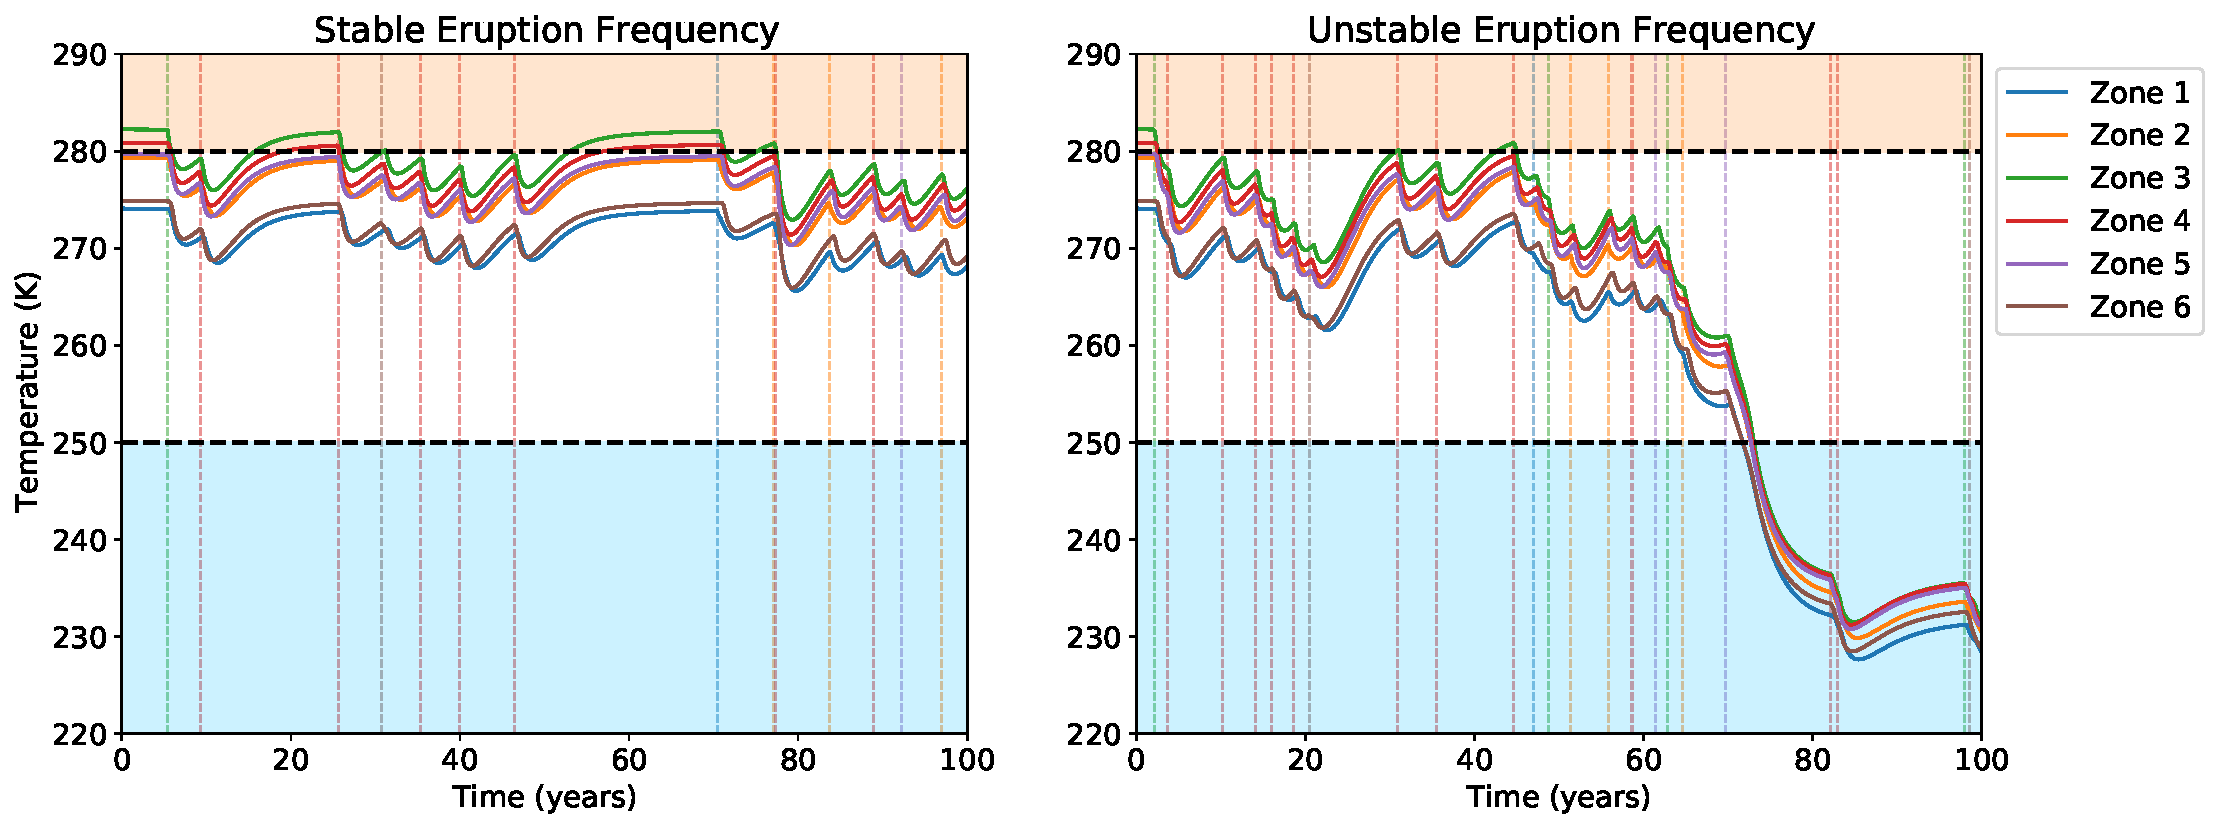
\includegraphics[width=\linewidth]{eruptions_albedo.pdf}
    \caption{
        Model results for volcanism combined with the ice-albedo feedback.
    }
    \label{fig:fireandice}
\end{figure}
\FloatBarrier

The stable eruption frequency model oscillates around the warm Earth equilibrium
shown in section \ref{sec:ice_albedo_results}. The unstable eruption frequency
oscillates around the warm Earth equilibrium for approximately
$70$ years before it quickly drops to oscillate around the snowball
Earth equilibrium.

\section{Discussion}

\subsection{Steady-State Climate Model: No Volcanism}
\label{section:steadystate}
The El Niño phenomena increases the rate of atmospheric and ocean
heat exchange allowing zonal temperatures to approach equilibrium more quickly.

\subsection{Volcanic Eruptions}
One of the aims of our study was to investigate the short-term impact of
volcanism on Earth's climate. The occlusion factor introduced in section
\ref{sec:Occlusion} ultimately acts to cool the climate by blocking direct
solar radiation from reaching the Earth's surface.\\

An interesting result is the difference in time scales for the occluding effect
of an eruption and the subsequent recovery time of the temperature. Figure
\ref{fig:occlusion} shows that suspended aerosols block less than 5\% of
direct solar radiation 2 years after an eruption. On the other hand, figure
\ref{fig:oneerupt} shows that it takes over a decade before zonal temperatures
recover to within 5\% of their equilibrium. This demonstrates volcanic aerosols
have an impact on the radiative energy balance of the Earth, even after the
aerosols have dissipated and are no longer blocking direct solar radiation.\\

The longer recovery time increases the susceptibility of the climate to compounding
temperature drops from multiple eruptions, as see in figure \ref{fig:stocherupt}.
Temperatures are forced to values over 10 degrees below their equilibrium values
during intense volcanic episodes. These high intensity volcanic
episodes can be a trigger that drives to Earth away from its initial equilibrium
into a snowball Earth state.

\subsection{The Ice-Albedo Effect}
The nonlinear albedo dependence on temperature defined in equation
\ref{eqn:albedoparam} ultimately gives rise to three equilibrium
conditions, as illustrated in figure \ref{fig:albedo_equil}. The ``warm Earth''
equilibrium represents conditions where the ice-albedo feedback has a small
effect on the Earth's global energy balance. Even when
temperatures fall in the variable albedo temperature range
(i.e. $250 \text{K} < T < 280 \text{K}$), no ice-albedo runaway is observed. \\

The ``snowball Earth'' equilibrium represents conditions where the ice-albedo
feedback has forced the Earth into a uniform, ice-covered state where each
zone has the characteristic albedo of ice. \\

Small changes in temperature near either of these equilibria are
compensated by a change in heat flow from adjacent
zones as well as a net imbalance of radiative energy fluxes which 
restores the temperatures to equilibrium. \\

The presence of two stable equilibria implies the existence of a third, unstable
equilibrium that separates the stable warm Earth and snowball Earth temperature
regimes. This unstable equilibrium arises as a consequence of the nonlinear albedo
dependence on temperature. A decrease in temperature near the unstable equilibrium
results in a sufficiently high increase in albedo where the reflected solar radiation
drives temperatures lower and further increases the albedo, resulting in a positive
feedback. \\

For a snowball Earth, the zonal albedo is constant, resulting a narrower
distribution of equilibrium temperatures. However, the higher heat transfer
coefficient between zones 4 and 5 maintains distinct equilibrium temperatures
for every zone.

\subsection{Fire and Ice: Stochastic Volcanism and the Ice-Albedo Feedback}
\label{sec:snowballearth}
Combining the cooling effects of volcanism with the ice-albedo feedback gives
a mechanism for driving the Earth away from its baseline, warm equilibrium.
We found that the Earth's temperatures are able to recover towards the warm Earth
equilibrium as long as volcanic eruption frequency
is low enough (represented by long repose times). If volcanic eruption
frequency is high enough (short repose times), the Earth's
temperatures drop below the critical unstable equilibrium temperatures, and
the runaway ice-albedo feedback drives the model to the snowball Earth equilibrium
(figure \ref{fig:fireandice}). \\

\subsection{Model Limitations} \label{sec:Limitations}
The Budyko climate model considered in this investigation greatly simplifies the
mechanics of heat exchange between latitudinal zones. In addition to the inherent
limitations of treating latitudinal heat exchange with constant conductivity coefficients,
a number of simplifications were made in our parameterization of volcanic eruptions. \\

The most important limitation is the absence of the heating effects of volcanism.
CO$_2$ is a significant component of volcanic emissions and is a strong greenhouse
gas. When present in the atmosphere, CO$_2$ re-emits outgoing long-wave radiation
back to the Earth's surface. This ultimately reduces the total outgoing radiation
from the Earth, resulting an increase in surface temperature. \\

As such, the accumulation of greenhouse gasses from volcanic eruptions may provide
a means to return to a warm Earth equilibrium by increasing surface temperatures above
the critical temperature threshold identified in our study. \\

Another limitation of our volcanic model is the assumption of a single eruption
type. A model that allows for a variation in eruption intensity and composition
would provide finer grain control over an eruption's impact the atmosphere and
its subsequent effects on Earth's surface temperatures. \\

We required an arbitrary increase in eruption rate frequencies to drive the Earth
to a snowball equilibrium. This is a consequence of modelling eruptions as a stationary
Poisson process. A non-stationary stochastic model of eruptions could allow for the clustering
of eruption activity as an alternative mechanism to trigger the runaway ice-albedo
feedback. \\

A limitation of our ice-albedo model is that as ice cover increases with dropping
temperatures, there may be an impact on atmospheric and oceanic heat circulation.
Our model does not parameterize these effects. For example, the heat transfer
coefficient, $k_{45}$, representing the El Niño phenomena in our model is constant,
though this value is likely dependent on the changing ocean and atmospheric interactions.


\section{Conclusion}
Inter-zonal heat transfer coefficients dictate the rate and efficiency of heat
distribution in our model. By implementing a stochastic eruption frequency
distribution as well as a nonlinear relationship between temperature and albedo,
we characterized the effect of volcanic activity on the global energy balance.
We found three equilibrium solutions, one being the snowball Earth state,
which can be approached through volcanism-induced temperature perturbations.
Our model parametrization, however, didn’t allow an escape from this new stable
state.

\subsection{Future Work}
As discussed in section \ref{sec:Limitations}, there are a number of ways our model
can be extended to consider different aspects of volcanism and its coupling with
ice-albedo feedback. A particularly interesting future direction to
consider would be the inclusion of the warming effect of volcano greenhouse gases.
In this way, volcanism can be studied as both a driving force to push Earth into
a snowball equilibrium as well as a way to recover from a snowball equilibrium.

\section{Ancillary Information}
\subsection{Author Contributions}

\begin{table}[H]
    \centering
    \begin{tabular}{rrr}
    Section & Subsection & Contributors \\
    \hline
    Graphic & Box-Model & M  \\
    Code & Steady-State Climate & P and E \\
    Code & Perturbation: Single Volcanic Eruption & P, E, and M \\
    Code & Snowball Earth & P, E, and M \\
    Introduction & Motivation & E and M \\
    Introduction & Budyko Climate Model & P \\
    Introduction & Direct Radiation Occlusion & P \\
    Introduction & Spatial Distribution of Aerosols & P \\
    Introduction & Ice-albedo Feedback & P \\ 
    Results & Steady-State Climate & M \\
    Results & Perturbation: Single Volcanic Eruption & M, E, P \\
    Results & Fire and Ice & M and P\\
    Discussion & Steady-State Climate Model & M \\
    Discussion & Perturbation: Single Volcanic Eruption & P \\
    Discussion & Fire and Ice & E, P, M\\
    Discussion & Model Limitations & E, P, M\\
    Conclusion & Future Work & E, M, and P \\
    Conclusion & Summary & E, M, and P \\
    \end{tabular}
    \caption{
        Contributions does not necessarily reflect discussion and preparation behind 
        concepts as this required continuous lateral communication between authors. 
        For example, all discussion sections were analyzed with
        input from each author, but written by
    }
    \label{tab:contributions}
\end{table}

\subsection{Algorithm Development} \label{sec:algorithm}

\begin{figure}[H]
    \centering
    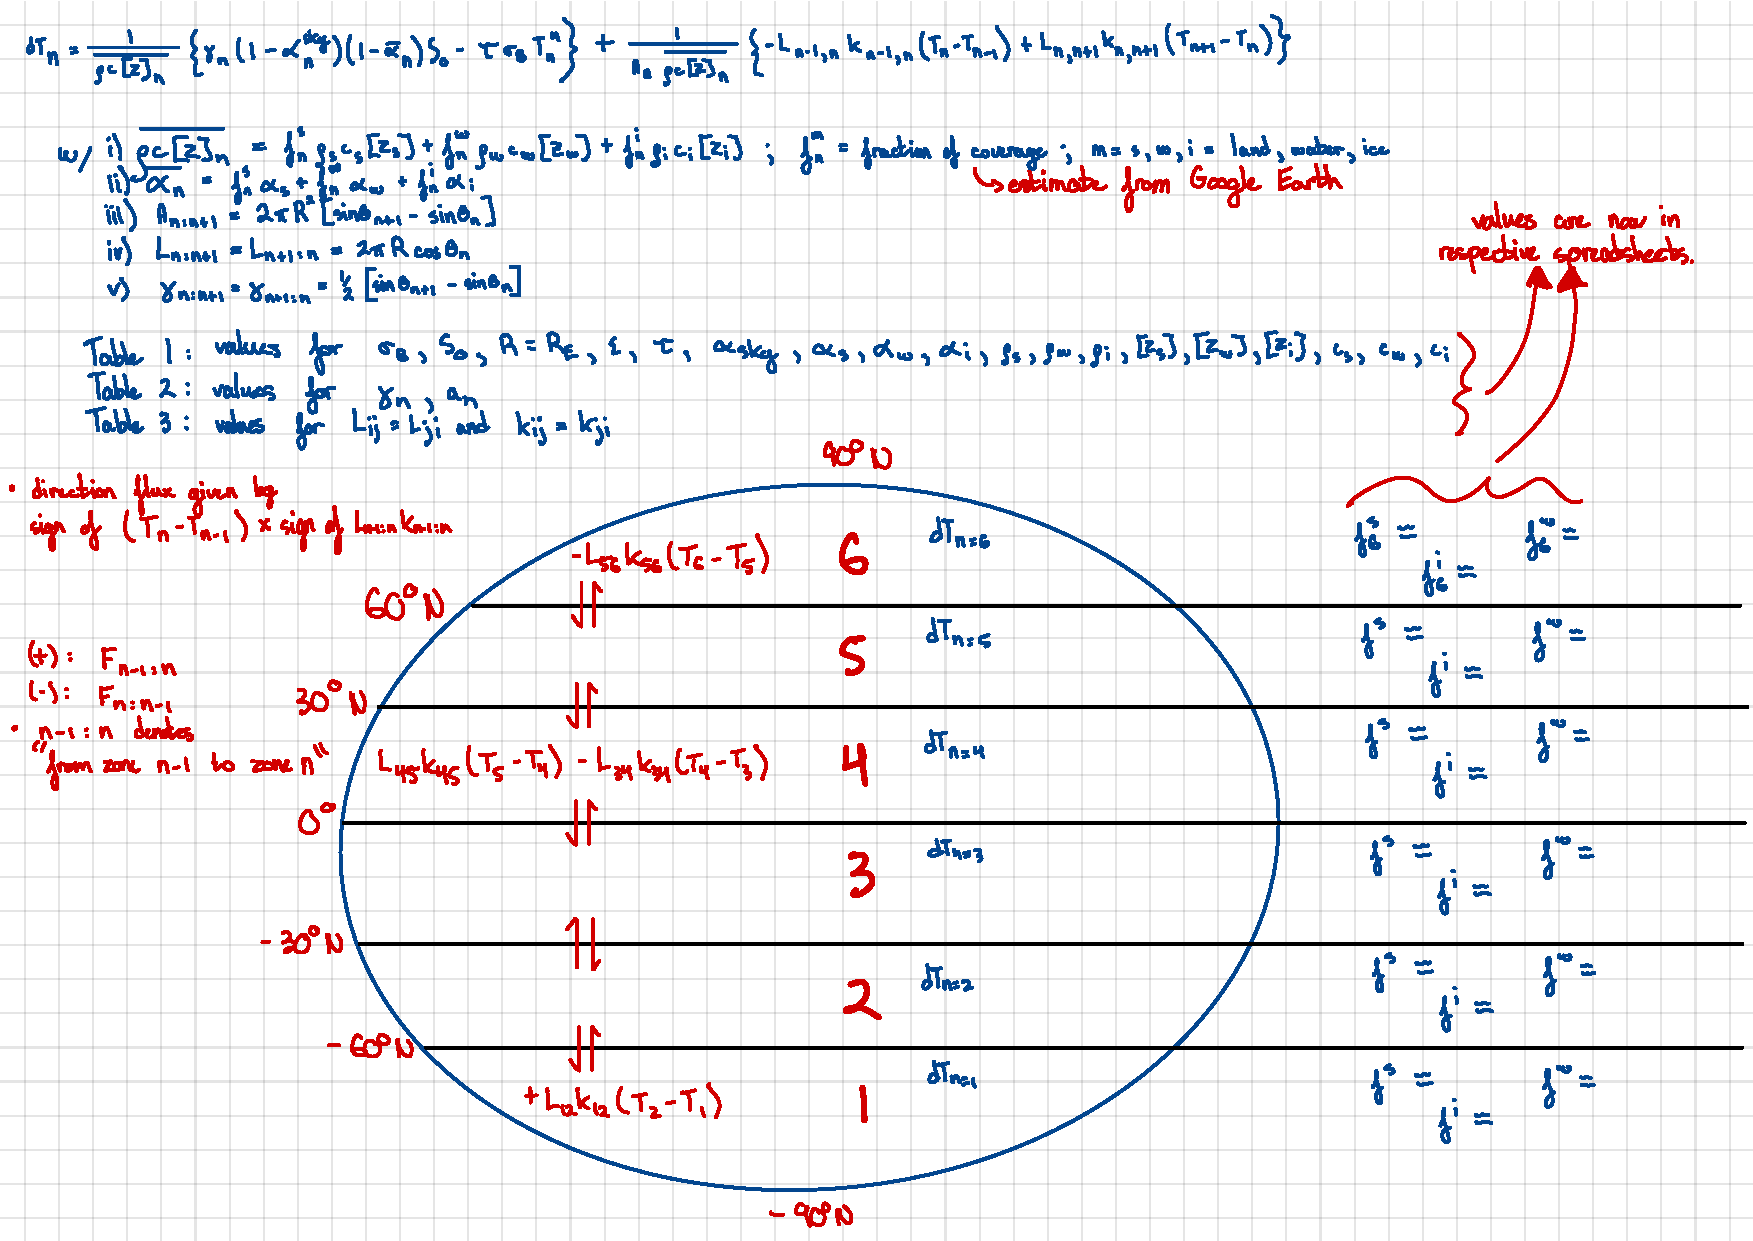
\includegraphics[scale=0.5]{Graphicalg.pdf}
    \caption{
        Sketch depicting zone intervals and necessary parameters for numerical
        solving.
    }
    \label{fig:graphicalg}
\end{figure}
\FloatBarrier

\subsection{Data}
\subsubsection{Eruption Times Series}
\begin{table}[H]
    \captionsetup{singlelinecheck = false, justification=justified}
    \caption{Eruption Times Series 1}
    \label{tab:erupt1}
    \begin{tabular}{c c}
    \hline
    Date & Direct Radiation [Wm$^{-2}$] \\
    \hline
    1982.39 & 347.03 \\
    1982.48 & 369.17 \\
    1982.56 & 384.44 \\
    1982.68 & 407.35 \\
    1982.82 & 439.42 \\
    1983.48 & 12.00 \\
    1983.60 & 488.30 \\
    1983.91 & 499.76 \\
    1984.63 & 506.66 \\
    1985.61 & 518.91 \\
    1986.36 & 521.23 \\
    1987.16 & 526.60 \\
    1988.53 & 64.00 \\
    1988.71 & 527.43 \\
    1990.38 & 525.96 \\
    1991.07 & 529.81 \\
    \hline
    \end{tabular}
\end{table}
\begin{table}[H]
    \captionsetup{singlelinecheck = false, justification=justified}
    \caption{Eruption Times Series 2}
    \label{tab:erupt2}
    \begin{tabular}{c c}
    \hline
    Date & Direct Radiation [Wm$^{-2}$] \\
    \hline
    1991.67 & 390.14 \\
    1991.87 & 412.28 \\
    1992.19 & 439.77 \\
    1992.45 & 464.21 \\
    1993.14 & 502.41 \\
    1993.83 & 516.94 \\
    1994.69 & 523.84 \\
    1995.72 & 527.69 \\
    1996.96 & 530.80 \\
    1998.05 & 532.36 \\
    1998.45 & 531.62 \\
    \hline
    \end{tabular}
\end{table}

\subsubsection{Parameters} \label{sec:Parameters}

\begin{table}[H]
    \captionsetup{singlelinecheck = false, justification=justified}
    \caption{Zonal Parameters}
    \begin{tabular}{llll}
    \hline
     & Parameter & Value \\
    \hline
    Zone 1 & Geometric Factor, $\gamma_1$ & 0.1076  \\
     & Area Fraction, $A_1$ & 0.067\\
     & Land Fraction, $f_1^s$ & 0.0 \\
     & Ocean Fraction, $f_1^w$  & 0.550925926 \\ 
     & Ice Fraction, $f_1^i$ & 0.449074074 \\
    \hline
    Zone 2 & Geometric Factor, $\gamma_2$ & 0.2277 \\
     & Area Fraction, $A_2$ & 0.183\\
     & Land Fraction, $f_2^s$ & 0.074074074 \\
     & Ocean Fraction, $f_2^w$ & 0.925925926 \\ 
     & Ice Fraction, $f_2^i$ & 0.0\\
    \hline
    Zone 3 & Geometric Factor, $\gamma_3$ & 0.3045 \\
     & Area Fraction, $A_3$ & 0.25 \\
     & Land Fraction, $f_3^s$ & 0.240740741 \\
     & Ocean Fraction, $f_3^w$ & 0.759259259 \\ 
     & Ice Fraction, $f_3^i$ & 0.0\\
    \hline
    Zone 4 & Geometric Factor, $\gamma_4$ & 0.3045 \\
     & Area Fraction, $A_4$ & 0.25 \\
     & Land Fraction, $f_4^s$ & 0.3101851851 \\
     & Ocean Fraction, $f_4^w$ & 0.689814815 \\ 
     & Ice Fraction, $f_4^i$ & 0.0 \\
    \hline
    Zone 5 & Geometric Factor, $\gamma_5$ & 0.2277 \\
     & Area Fraction, $A_5$ & 0.183 \\
     & Land Fraction, $f_5^s$ & 0.694444444 \\
     & Ocean Fraction, $f_5^w$ & 0.305555556 \\ 
     & Ice Fraction, $f_5^i$ & 0.0 \\
    \hline
    Zone 6 & Geometric Factor, $\gamma_6$ & 0.1076\\
     & Area Fraction, $A_6$ & 0.067 \\
     & Land Fraction, $f_6^s$ & 0.277777778\\
     & Ocean Fraction, $f_6^w$  & 0.652777778\\ 
     & Ice Fraction, $f_6^i$ & 0.069444444\\
    \end{tabular}
    \label{tab:zoneparams}
\end{table}
\FloatBarrier

\begin{table}
    \captionsetup{singlelinecheck = false, justification=justified}
    \caption{Global Parameters}
    \begin{tabular}{lll}
    \hline
    Parameter & Value & Units\\
    \hline
    Stefan-Boltzmann Constant, $\sigma_B$ & 5.6696e-8 & $Wm^{-2}K^{-4}$ \\
    Solar Constant, $S_0$ & 1368 & $Wm^{-2}$ \\
    Earth Radius, $R_E$ & 6371e3 & $m$ \\
    Earth Total Emissivity, $\epsilon$  & 1  \\
    Surface Area of Earth, $A_E$ & $\pi R_E^2$ & $m^2$ \\
    Atmospheric Transmissivity, $\tau$ & 0.63  \\
    Atmospheric Albedo, $\alpha_{sky}$ & 0.2 \\
    Land Albedo, $\alpha_s$ & 0.4 \\
    Ocean Albedo, $\alpha_w$ & 0.1\\
    Ice Albedo, $\alpha_i$ & 0.6 \\
    Land Density, $\rho_s$ & 2500 & $kgm^{-3}$\\
    Ocean Density, $\rho_w$ & 1028 & $kgm^{-3}$\\
    Ice Density, $\rho_i$ & 900 & $kgm^{-3}$\\
    Land Thermal Scale Depth, $[Z_s]$ & 1.0 & $m$ \\
    Ocean Thermal Scale Depth, $[Z_w]$ & 70.0 & $m$ \\
    Ice Thermal Scale Depth, $[Z_i]$ & 1.0 & $m$ \\
    Land Specific Heat Capacity, $c_s$ & 790 & $JkgK^{-1}$\\
    Ocean Specific Heat Capacity, $c_w$ & 4187 & $JkgK^{-1}$\\
    Ice Specific Heat Capacity, $c_i$ & 2060 & $JkgK^{-1}$\\
    \end{tabular}
    \label{tab:globalparams}
\end{table}
\FloatBarrier

\begin{table}
    \captionsetup{singlelinecheck = false, justification=justified}
    \caption{Boundary Parameters}
    \begin{tabular}{lll}
    \hline
    Parameter & Value & Units\\
    \hline
    Boundary 12 ($60^{\circ}S)$ & & \\
    Boundary Length, $L_{12}$ & 2.0015e7 & $m$ \\
    Thermal exchange coefficient, $k_{12}$ & 1e7 & $Wm^{-1}K^{-1}$ \\ 
    Boundary 23 ($30^{\circ}S)$ & & \\
    Boundary Length, $L_{23}$ & 3.4667e7 & $m$ \\
    Thermal exchange coefficient, $k_{23}$ & 1e7 & $Wm^{-1}K^{-1}$ \\
    Boundary 34 ($0^{\circ}S)$ & & \\
    Boundary Length, $L_{34}$ & 4.0030e7 & $m$ \\
    Thermal exchange coefficient, $k_{34}$ & 1e7 & $Wm^{-1}K^{-1}$ \\ 
    Boundary 45 ($30^{\circ}N)$ & & \\
    Boundary Length, $L_{45}$ & 3.4667e7 & $m$ \\
    Thermal exchange coefficient, $k_{45}$ & 5e7 & $Wm^{-1}K^{-1}$ \\
    Boundary 56 ($60^{\circ}N)$ & & \\
    Boundary Length, $L_{56}$ & 2.0015e7 & $m$ \\
    Thermal exchange coefficient, $k_{56}$ & 1e7 & $Wm^{-1}K^{-1}$ \\
    \end{tabular}
    \label{tab:boundaryparams}
\end{table}
\FloatBarrier

\newpage
\printbibliography

\end{document}
